% !TEX TS-program = XeLaTeX
% use the following command:
% all document files must be coded in UTF-8
\documentclass[portuguese]{textolivre}
% build HTML with: make4ht -e build.lua -c textolivre.cfg -x -u article "fn-in,svg,pic-align"

\journalname{Texto Livre}
\thevolume{18}
%\thenumber{1} % old template
\theyear{2025}
\receiveddate{\DTMdisplaydate{2025}{4}{7}{-1}} % YYYY MM DD
\accepteddate{\DTMdisplaydate{2025}{5}{18}{-1}}
\publisheddate{\DTMdisplaydate{2025}{6}{18}{-1}}
\corrauthor{Júlio Araújo}
\articledoi{10.1590/1983-3652.2025.58505}
%\articleid{NNNN} % if the article ID is not the last 5 numbers of its DOI, provide it using \articleid{} commmand 
% list of available sesscions in the journal: articles, dossier, reports, essays, reviews, interviews, editorial
\articlesessionname{essays}
\runningauthor{Araújo} 
%\editorname{Leonardo Araújo} % old template
\sectioneditorname{Daniervelin Pereira}
\layouteditorname{Leonado Araújo}

\title{O algoritmo é um texto}
\othertitle{The algorithm is a text}
% if there is a third language title, add here:
%\othertitle{Artikelvorlage zur Einreichung beim Texto Livre Journal}

\author[1]{Júlio Araújo~\orcid{0000-0001-7399-3769}\thanks{Email: \href{mailto:araujo@ufc.br}{araujo@ufc.br}}}
\affil[1]{Universidade Federal do Ceará, Programa de Pós-Graduação em Linguística, Fortaleza, CE, Brasil.}

\addbibresource{article.bib}
% use biber instead of bibtex
% $ biber article

% used to create dummy text for the template file
\definecolor{dark-gray}{gray}{0.35} % color used to display dummy texts
\usepackage{lipsum}
\SetLipsumParListSurrounders{\colorlet{oldcolor}{.}\color{dark-gray}}{\color{oldcolor}}

% used here only to provide the XeLaTeX and BibTeX logos
\usepackage{hologo}

% if you use multirows in a table, include the multirow package
\usepackage{multirow}

% provides sidewaysfigure environment
\usepackage{rotating}

% CUSTOM EPIGRAPH - BEGIN 
%%% https://tex.stackexchange.com/questions/193178/specific-epigraph-style
\usepackage{epigraph}
\renewcommand\textflush{flushright}
\makeatletter
\newlength\epitextskip
\pretocmd{\@epitext}{\em}{}{}
\apptocmd{\@epitext}{\em}{}{}
\patchcmd{\epigraph}{\@epitext{#1}\\}{\@epitext{#1}\\[\epitextskip]}{}{}
\makeatother
\setlength\epigraphrule{0pt}
\setlength\epitextskip{0.5ex}
\setlength\epigraphwidth{.7\textwidth}
% CUSTOM EPIGRAPH - END

% to use IPA symbols in unicode add
%\usepackage{fontspec}
%\newfontfamily\ipafont{CMU Serif}
%\newcommand{\ipa}[1]{{\ipafont #1}}
% and in the text you may use the \ipa{...} command passing the symbols in unicode

% LANGUAGE - BEGIN
% ARABIC
% for languages that use special fonts, you must provide the typeface that will be used
% \setotherlanguage{arabic}
% \newfontfamily\arabicfont[Script=Arabic]{Amiri}
% \newfontfamily\arabicfontsf[Script=Arabic]{Amiri}
% \newfontfamily\arabicfonttt[Script=Arabic]{Amiri}
%
% in the article, to add arabic text use: \textlang{arabic}{ ... }
%
% RUSSIAN
% for russian text we also need to define fonts with support for Cyrillic script
% \usepackage{fontspec}
% \setotherlanguage{russian}
% \newfontfamily\cyrillicfont{Times New Roman}
% \newfontfamily\cyrillicfontsf{Times New Roman}[Script=Cyrillic]
% \newfontfamily\cyrillicfonttt{Times New Roman}[Script=Cyrillic]
%
% in the text use \begin{russian} ... \end{russian}
% LANGUAGE - END

% EMOJIS - BEGIN
% to use emoticons in your manuscript
% https://stackoverflow.com/questions/190145/how-to-insert-emoticons-in-latex/57076064
% using font Symbola, which has full support
% the font may be downloaded at:
% https://dn-works.com/ufas/
% add to preamble:
% \newfontfamily\Symbola{Symbola}
% in the text use:
% {\Symbola }
% EMOJIS - END

% LABEL REFERENCE TO DESCRIPTIVE LIST - BEGIN
% reference itens in a descriptive list using their labels instead of numbers
% insert the code below in the preambule:
%\makeatletter
%\let\orgdescriptionlabel\descriptionlabel
%\renewcommand*{\descriptionlabel}[1]{%
%  \let\orglabel\label
%  \let\label\@gobble
%  \phantomsection
%  \edef\@currentlabel{#1\unskip}%
%  \let\label\orglabel
%  \orgdescriptionlabel{#1}%
%}
%\makeatother
%
% in your document, use as illustraded here:
%\begin{description}
%  \item[first\label{itm1}] this is only an example;
%  % ...  add more items
%\end{description}
% LABEL REFERENCE TO DESCRIPTIVE LIST - END


% add line numbers for submission
%\usepackage{lineno}
%\linenumbers

\begin{document}
\maketitle

\begin{polyabstract}
\begin{abstract}
Neste ensaio, defendo que os algoritmos podem e devem ser lidos como textos performativos, cujas ações discursivas organizam sentidos, moldam interações e impactam práticas sociais. A partir de uma concepção contemporânea da Linguística Textual, que compreende o texto como atividade situada, interacional, cognitiva e multimodal \cite{koch2006,marcuschi2008,beaugrande1997}, argumento que os algoritmos não são apenas instruções codificadas, mas formas de textualização que exercem poder simbólico e pragmático no mundo. Para sustentar essa hipótese, analiso duas simulações algorítmicas escritas em linguagem de programação: um modelo de preparo de café e um sistema de recomendação de conteúdo em plataformas de \textit{streaming}. Nessas análises, demonstro como fatores de textualidade como coesão, coerência, intencionalidade, aceitabilidade, informatividade, situacionalidade e intertextualidade se realizam como efeitos emergentes de processos comunicativos mediados por código. Ao deslocar o foco dos critérios estruturais para os modos de produção de sentido, mostro que os algoritmos não apenas compartilham traços textuais com os discursos humanos, mas também produzem interpretações, respostas e experiências. Concluo que reconhecer os algoritmos como textos permite submetê-los a uma leitura crítica e ética, capaz de revelar suas ideologias embutidas e reivindicar a transparência e reescrita dos códigos que orientam a vida digital contemporânea.

\keywords{Algoritmo \sep Textualidade \sep Inteligência Artificial}
\end{abstract}

\begin{english}
\begin{abstract}
In this essay, I argue that algorithms can and should be read as performative texts, whose discursive actions organize meaning, shape interaction, and impact social practices. Drawing on a contemporary framework of Text Linguistics, which understands text as a situated, intersubjective, cognitive, and multimodal activity \cite{koch2006,marcuschi2008,beaugrande1997}, I maintain that algorithms are not merely coded instructions, but forms of textualization that exert symbolic and pragmatic power in the digital world. To support this hypothesis, I analyze two algorithmic simulations written in programming language: a coffee-making model and a content recommendation system for streaming platforms. Through these analyses, I demonstrate how textuality factors such as cohesion, coherence, intentionality, acceptability, informativeness, situationality, and intertextuality emerge as effects of communication processes mediated by code. By shifting the focus from structural criteria to meaning-making dynamics, I show that algorithms not only share textual features with human discourse, but also generate interpretations, responses, and experiences. I conclude that recognizing algorithms as texts enables us to submit them to critical and ethical scrutiny, capable of revealing embedded ideologies and demanding transparency and the rewriting of the codes that shape contemporary digital life.

\keywords{Algorithm \sep Textuality \sep Artificial Intelligence}
\end{abstract}
\end{english}
% if there is another abstract, insert it here using the same scheme
\end{polyabstract}

\section{Introdução}\label{sec-intro}
Na era da inteligência artificial, os algoritmos tornaram-se escribas invisíveis, moldando narrativas que estruturam nosso cotidiano. Como linguagens que operam sob o disfarce da neutralidade técnica, eles escrevem o presente a partir de comandos invisíveis, modelando o que é visível e o que permanece oculto nos fluxos digitais de informação. De mecanismos de busca à personalização do consumo cultural, eles não apenas organizam dados, mas constroem realidades, influenciando o que vemos, sabemos e até quem somos. Apesar disso, a linguagem algorítmica é comumente tratada como técnica e neutra, ocultando sua dimensão discursiva. Ainda se acredita que algoritmos sejam apenas sequências formais de comandos, desprovidas de intencionalidade e sentido.

Este ensaio contesta essa visão reducionista, ao defender que os algoritmos são textos e, por isso, eles operam performatividades, uma vez que organizam sentidos, geram respostas e regulam interações. Assim como um texto articula elementos linguísticos, cognitivos e situacionais para fazer sentido, os algoritmos produzem efeitos discursivos que moldam a experiência digital. A textualidade algorítmica, nesse sentido, não está em propriedades fixas, mas em processos emergentes de significação, mediados por código, interface, contexto e leitura.

Essa abordagem se ancora nas reformulações contemporâneas propostas por \textcite{beaugrande1997,koch2006,marcuschi2008}, que entendem o texto como prática social, cognitiva e multimodal. Com base nisso, pergunto: o que se revela quando observamos o algoritmo por meio da lente da textualidade? Essa questão é relevante porque circunscrever o algoritmo apenas à condição técnica e matemática é insuficiente para explicar o modo como a inteligência artificial opera nas práticas discursivas contemporâneas. Ao mobilizar a textualidade como lente de análise, proponho deslocar o olhar do funcionamento computacional para as operações discursivas que sustentam e legitimam esses sistemas. A textualidade, entendida em sua dimensão cognitiva, interacional e multimodal, permite reconhecer os algoritmos como artefatos produtores de linguagem, dotados de intencionalidade comunicativa e efeitos pragmáticos.

Perguntar o que se revela nessa travessia conceitual é afirmar que há muito mais nos algoritmos do que instruções técnicas, já que eles plasmam discurso, poder e disputa simbólica. Para investigar a referida questão, mobilizo os fatores de textualidade consagrados por \textcite{halliday1976,beaugrande1981} não como critérios normativos, mas como dimensões que emergem nos processos de textualização.

Para sustentar essa argumentação, apresento a análise de dois exemplos simulados em linguagem de programação: um algoritmo de preparo de café e um sistema de recomendação em plataformas de \textit{streaming}. Em vez de verificar o cumprimento de critérios formais, a proposta é ler esses algoritmos como enunciados performativos, em que as operações de sentido dependem de encadeamentos, inferências, contexto, repetição, aprendizado e interação com o usuário.

No contexto deste ensaio, afirmar que o algoritmo é um texto não é mero exercício conceitual de deslocamento epistemológico, mas um gesto político e ético. Se os algoritmos produzem linguagem, então podem e devem ser submetidos à crítica discursiva. É preciso perguntar quem os escreve, com que gramática simbólica, sob quais interesses e contra quais corpos, para compreender que os algoritmos não são apenas ferramentas, mas formas de governo das condutas. Diante do racismo algorítmico, das bolhas informacionais e das decisões automatizadas que afetam vidas, compreendê-los como textos é reivindicar o direito de lê-los criticamente e, sobretudo, de reescrevê-los como forma de justiça discursiva.

\section{Quando o código escreve o mundo: definições e disputas}\label{sec-normas}
Um algoritmo é uma sequência finita de instruções claras e não ambíguas, destinadas a resolver um problema ou executar uma tarefa. Cada etapa é seguida de forma sistemática para garantir o resultado esperado. Por exemplo, um algoritmo de controle de temperatura em sistemas de aquecimento residencial pode ser representado por um fluxo lógico de entrada de dados, processamento, tomada de decisão, repetição, saída e término, etapas essenciais que ilustram sua operação automatizada e lógica. Esse processo pode ser representado visualmente por meio de fluxogramas simples, como ilustrado na \Cref{fig1}.

A \Cref{fig1} mostra o funcionamento de um algoritmo de controle de temperatura, com suas principais etapas. O processo começa com a entrada de dados, obtidos por sensores internos da residência. Em seguida, o algoritmo processa essas informações e decide a ação a ser tomada com base na temperatura ambiente. A decisão segue uma lógica condicional: se a temperatura estiver abaixo do limite, o aquecimento é ativado; se ultrapassar, é desligado; e, se estiver dentro da faixa ideal, o sistema permanece como está. Essa estrutura evidencia a lógica dos algoritmos de automação.

Um elemento central nesse tipo de algoritmo é o laço de repetição, que atualiza continuamente as leituras de temperatura e permite a adaptação às variações do ambiente. Esse monitoramento constante impede que o sistema fique em estado fixo, garantindo eficiência e controle dinâmico. A etapa seguinte, de saída, corresponde ao ajuste no estado do aquecimento e à comunicação do status: ligado, desligado ou inalterado.

O algoritmo se encerra quando o sistema é desativado manualmente ou por uma condição de parada predefinida. Essa estrutura sequencial reflete a lógica automatizada do processo, demonstrando como os algoritmos aplicam princípios de eficiência e controle para otimizar o consumo energético e garantir o conforto térmico. A \Cref{fig1} ilustra essa integração entre código e sistema físico, evidenciando o papel dos algoritmos na inteligência computacional e na gestão de recursos.

\begin{figure}[h!]
    \centering
    \begin{minipage}{0.5\linewidth}
    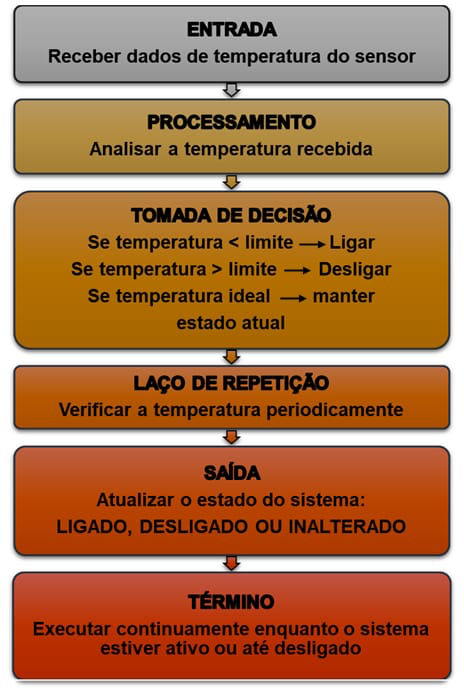
\includegraphics[width=\linewidth]{Fig1.png}
    \caption{Fluxo de funcionamento de um algoritmo de controle de temperatura em sistemas de aquecimento residencial.}
    \label{fig1}
    \source{Elaborado pelo autor via simulação por IA.}
    \end{minipage}
\end{figure}

À luz do exemplo apresentado, pode-se definir o algoritmo como uma estrutura lógica e finita de instruções que transforma entradas em saídas, mediando a relação entre um problema e sua solução. Funciona como um texto processual, em que cada passo determina ações ordenadas e condicionais. Assim, não se trata apenas de comandos executáveis, mas de um sistema de organização de dados e decisões, capaz de automatizar soluções e adaptar-se a diferentes contextos.

Presentes em diversos campos do conhecimento, os algoritmos são conjuntos de instruções bem definidas para resolver problemas e automatizar tarefas. Na ciência da computação, configuram-se como sequências finitas de ações voltadas à solução de problemas \cite{setzer1992}. Nas linguagens de programação, assumem a forma de códigos estruturados, com sintaxe e semântica específicas \cite{ludermir2021}. Já na inteligência artificial, são projetados para reconhecer padrões em grandes volumes de dados, permitindo que sistemas aprendam e tomem decisões autonomamente \cite{alhasnawi2024}.

Embora comumente apresentados como ferramentas neutras, algoritmos operam como estruturas de controle com implicações epistemológicas e discursivas. É o que propõe \textcite{hill2016}, ao ampliar o entendimento tradicional com uma definição que rompe com a visão mecanicista, pois, segundo ela, “um algoritmo é uma \emph{estrutura de controle composta}, \emph{finita}, \emph{abstrata} e \emph{efetiva}, dada de forma \emph{imperativa}, que \emph{realiza um propósito específico} sob condições previamente estabelecidas”\footnote{Tradução livre de: “An algorithm is a finite, abstract, effective, compound control structure, imperatively given, accomplishing a given purpose under given provisions”.} \cite[p. 47, grifos nossos, tradução nossa]{hill2016}.

Essa definição amplia a compreensão tradicional dos algoritmos, atribuindo-lhes um \textit{status} ontológico: não são apenas descrições formais de processos computacionais, mas entidades estruturadas que impõem regras e operam dentro de condições específicas. Para \textcite{hill2016}, um algoritmo deve ser entendido a partir de seis características fundamentais:

\begin{enumerate}
    \item \emph{Finito} – Um algoritmo deve ter uma representação expressável em um espaço e tempo finito.
    \item \emph{Abstrato} – Ele não está vinculado a uma manifestação física específica, podendo ser aplicado em diferentes contextos.
    \item \emph{Efetivo} – Deve ser executável sem exigir julgamento humano, intuição ou criatividade.
    \item \emph{Estruturado} – Consiste em uma sequência organizada de operações que determinam como uma ação será realizada.
    \item \emph{Imperativo} – Deve prescrever ações de forma clara e não ambígua.
    \item \emph{Intencional} – Cada algoritmo é projetado para alcançar um propósito específico dentro de determinadas condições.
\end{enumerate}
   
Essas propriedades não apenas descrevem a mecânica do algoritmo, mas indicam sua função organizadora, tal como os textos, ao estabelecer sequências, propósitos e efeitos comunicativos. \textcite{hill2016} propõe que um algoritmo não se resume ao código ou à implementação, pois sua identidade transcende qualquer forma específica de escrita. Trata-se de um conceito mais amplo, que regula processos, estabelece ordens e define condições de funcionamento. Essa definição permite uma analogia direta entre algoritmos e textos, pois ambos são estruturas organizadas para produzir sentido em um contexto determinado. O algoritmo, assim, funciona como uma estrutura discursiva que gera significação ao processar dados e produzir saídas com impacto na realidade.

Como qualquer texto pode ser analisado por sua sintaxe, semântica e pragmática, os algoritmos também devem ser compreendidos como construções discursivas que carregam intenções, pressupostos e efeitos políticos e sociais. \textcite{hill2016} reforça essa perspectiva ao afirmar que os algoritmos não são meros mecanismos matemáticos, mas entidades com implicações epistemológicas, uma vez que eles impõem lógicas, modelam interações e funcionam como narrativas estruturadas que organizam o mundo.

O PageRank\footnote{O PageRank é um algoritmo criado por Larry Page e Sergey Brin para medir a relevância de páginas na web com base na quantidade e qualidade dos links que apontam para elas. O algoritmo assume que páginas referenciadas por outras páginas importantes são mais relevantes, influenciando o ranqueamento nos resultados de busca do Google \cite{brin1998}.}, algoritmo de ranqueamento do Google, exemplifica como algoritmos não apenas ordenam informações, mas hierarquizam relevâncias e regulam visibilidades. Tal como um texto, estabelece critérios de leitura do mundo digital, definindo o que será mais ou menos acessível. Assim, o algoritmo atua como instrumento discursivo de poder, pois, como afirma \textcite{hill2016}, ele “é uma estrutura de controle” que seleciona, exclui e enfatiza determinadas realidades.

Um aspecto central destacado por \textcite{hill2016} é a imperatividade do algoritmo. Ao dizer que ele é “imperativamente dado”, a autora indica que se trata de um conjunto de instruções que prescreve ações, e não de uma simples descrição de caminhos possíveis. Esse caráter prescritivo insere os algoritmos no cerne de debates políticos e éticos. Em muitos contextos, eles operam como mecanismos invisíveis de regulação social, pois determinam quem tem acesso a crédito \cite{loya2022}, quem recebe tratamento de saúde \cite{onwuegbuzia2024}, quais anúncios são exibidos \cite{farries2024} e que discursos são amplificados ou silenciados \cite{garcia2021}. Essa lógica algorítmica, mais do que organizar dados, hierarquiza relações sociais, frequentemente de forma opaca e excludente.

O racismo algorítmico exemplifica o poder imperativo dos algoritmos. Sistemas de inteligência artificial treinados com dados enviesados tendem a reproduzir desigualdades históricas, perenizando discriminações raciais em processos como recrutamento, concessão de crédito, policiamento preditivo e reconhecimento facial \cite{silva2022}.

Essas decisões não são meramente técnicas, mas atos de escrita sobre o mundo, que operam como enunciados performativos e produzem efeitos materiais e simbólicos naquilo que denomino sociedade da necroalgoritmização \cite{araujo2025_necroalgoritmizacao}. Ao entender essas decisões como discursos automatizados, torna-se ainda mais urgente o desenvolvimento de metodologias críticas de leitura e contestação.

A definição de \textcite{hill2016} nos convida a compreender os algoritmos como entidades discursivas estruturadas que, além de processar dados, produzem sentido e impacto social. Se, como afirma a autora, o algoritmo é uma “estrutura abstrata, efetiva e imperativa”, então deve ser analisado criticamente como qualquer texto que organiza a realidade social.

Em função disso, a tese de que o algoritmo é um texto amplia esse entendimento ao mostrar que ele constrói narrativas sobre o mundo, define quais informações circulam, quem é reconhecido e quais decisões são tomadas. Como todo texto, carrega pressupostos, intenções e ideologias. Por isso, sua leitura crítica é essencial para evitar que reforcem injustiças.

Se os algoritmos são estruturas discursivas de poder, é preciso lê-los, interpretá-los e reescrevê-los. Isso implica exigir transparência, regulação e participação social em sua construção, além de desenvolver métodos de auditoria e contestação. Em última instância, afirmar que o algoritmo é um texto é reivindicar o direito de recontar a história que os algoritmos escrevem sobre nós.

Ao compreender os algoritmos como estruturas discursivas performativas, torna-se possível pensar sua análise não como um exercício técnico, mas como um gesto de leitura crítica. E se o algoritmo é um texto, ele também é passível de escuta, interpretação, réplica. É a partir dessa hipótese que passo a articular sua leitura com os fundamentos clássicos e atuais da Linguística Textual.

\section{Da coesão à ação: o texto além das frases}\label{sec-fmt-manuscrito}
O conceito de texto, na Linguística Textual, deixou de ser visto como um simples encadeamento de sentenças para ser compreendido como uma unidade discursiva situada em contextos comunicativos. \textcite{jakobson1960} relaciona a textualidade às funções da linguagem; \textcite{barthes1978} destaca a intertextualidade como princípio organizador do sentido. \textcite{halliday1976} introduzem a coesão e a coerência como elementos estruturantes do texto, enquanto \textcite{beaugrande1981} ampliam essa concepção ao incorporar dimensões pragmáticas, interativas e contextuais. A partir dessas concepções, proponho que algoritmos possam ser analisados não como códigos operacionais isolados, mas como textos que constroem sentidos e regulam práticas sociais.

Em \textit{Cohesion in English}, \textcite[p. 1, tradução nossa]{halliday1976}\footnote{Tradução livre de: “a unit of language in use […] not a grammatical unit, but rather a semantic unit”.} definem o texto como “uma unidade da língua em uso” e ressaltam que ele não é “uma unidade gramatical, mas sim uma unidade semântica”. Essa perspectiva destaca a função do texto na comunicação, sustentada por mecanismos estruturais que garantem sua significação. A coesão refere-se às conexões linguísticas explícitas, como referência, substituição, elipse e conectores, enquanto a coerência diz respeito à articulação lógica e semântica entre as ideias, apoiada pelo conhecimento de mundo dos interlocutores.

\textcite{beaugrande1981}, em \textit{Introduction to Text Linguistics}, ampliam o modelo de Halliday e Hasan ao propor cinco novos critérios de textualidade: intencionalidade, aceitabilidade, informatividade, situacionalidade e intertextualidade. Para eles, o texto não é apenas uma sequência de sentenças, mas uma ocorrência comunicativa situada, cujos sentidos emergem da interação entre estrutura, contexto e intenção comunicativa. Essa virada teórica reposiciona o texto como uma prática discursiva processual, que se atualiza nas relações entre estrutura, contexto e intenção comunicativa. Assim, o texto passa a ser concebido como um evento discursivo dinâmico, influenciado por fatores pragmáticos e sociais.

A proposta de \textcite{beaugrande1981} não apenas retoma a centralidade da coesão e da coerência defendida por \textcite{halliday1976}, mas amplia o conceito de texto ao incluir dimensões contextuais e pragmáticas. Para os autores, o texto está ligado ao propósito comunicativo (intencionalidade), à recepção dos interlocutores (aceitabilidade) e às relações com outros discursos (intertextualidade).

Essa perspectiva sustenta minha tese de que algoritmos podem ser compreendidos como textos. Ao aplicar os critérios de textualidade aos algoritmos, reconhecemos que eles não são apenas estruturas formais (coesão), mas também fenômenos discursivos atravessados por coerência, intencionalidade, aceitabilidade, informatividade, situacionalidade e intertextualidade. Essa compreensão dialógica da textualidade converge com a definição proposta por \textcite{hill2016}, que define o algoritmo como uma estrutura composta, abstrata e finita, criada para cumprir um propósito específico. Para a autora, os algoritmos envolvem não apenas formulações formais, mas também aspectos contextuais e processuais. Assim, analisá-los como textos é reconhecê-los como eventos comunicativos situados, marcados por intencionalidade e função discursiva.

Com base nessa ampliação, argumento que os critérios de textualidade propostos por \textcite{halliday1976,beaugrande1981} oferecem caminhos relevantes para compreender os algoritmos em sua complexidade discursiva. Contudo, tais fatores não operam como exigências universais, mas como dimensões possíveis de análise, que devem ser observadas à luz do funcionamento interacional e sociotécnico dos algoritmos. Se o texto é uma ocorrência comunicativa ancorada em um contexto e organizada por relações estruturais e funcionais, então os algoritmos, ao estruturar informações, operar com lógica formal e interagir com sistemas e usuários, cumprem essa mesma função textual e comunicativa.

Proponho, portanto, um deslocamento de olhar: em vez de tratar o algoritmo apenas como instrução técnica, passo a analisá-lo como fenômeno textual, produtor de sentidos e inserido em redes intertextuais. Nos tópicos seguintes, apresento como cada critério de textualidade se manifesta na lógica algorítmica, reforçando a ideia de que o algoritmo é, em essência, um texto.


\section{Costurando comandos: a coesão como operação simbólica}\label{sec-formato}
A noção de coesão tem sido tradicionalmente compreendida como um conjunto de mecanismos linguísticos que conectam formalmente as partes de um texto, assegurando sua continuidade e inteligibilidade. Essa formulação, apresentada por \textcite{halliday1976}, foi decisiva para o surgimento da Linguística Textual como campo, mas vem sendo reformulada por abordagens mais recentes. \textcite{koch2006}, por exemplo, propõe que a coesão não é um critério fixo, mas um fator que pode ou não ser ativado em diferentes situações de textualização, dependendo do contexto, do suporte e da finalidade comunicativa. \textcite{marcuschi2008}, por sua vez, destaca que a coesão pode se manifestar em diferentes modos semióticos, por imagens, sons, ícones ou sequências visuais, sobretudo em textos digitais e multimodais.

No caso dos algoritmos, a coesão textual não é apenas uma estrutura interna do código, uma vez que  ela se expressa na forma como os elementos algorítmicos se articulam funcional e discursivamente. Diante da opacidade que envolve os algoritmos reais, muitas vezes protegidos por “segredos comerciais vitais” \cite[p. 208]{oneil2020} e marcados por uma “performance invisível” \cite[p. 12]{santaella2023}, proponho um experimento textual: a simulação de um algoritmo de preparo de café, escrito em linguagem de programação. Essa simulação, longe de ser meramente ilustrativa, permite observar como a textualidade algorítmica se constrói como prática processual, interacional e situada, ativando fatores cognitivos, estratégias de previsibilidade e modos de apresentação multimodal.

A análise do código (\Cref{fig2}) que segue busca demonstrar como tais elementos configuram o algoritmo como texto performativo e interpretável, conforme as abordagens contemporâneas da Linguística Textual \cite{koch2006,marcuschi2008,beaugrande1997}.


\begin{lstlisting}[language=Python, label=fig2, caption={Algoritmo de preparo de café representado em linguagem de programação.}, source={Elaborado pelo autor via simulação por IA.}]
def fazer_cafe():
    aquecer_agua()
    adicionar_cafe()
    adicionar_acucar()
    misturar()

def aquecer_agua():
    print("Aquecendo a água até 90°C.")

def adicionar_cafe():
    print("Adicionando café ao filtro.")

def adicionar_acucar():
    print("Adicionando açúcar a gosto.")

def misturar():
    print("Misturando a bebida.")

# Executando o algoritmo
fazer_cafe()
\end{lstlisting}
% \begin{figure}[h!]
%     \centering
%     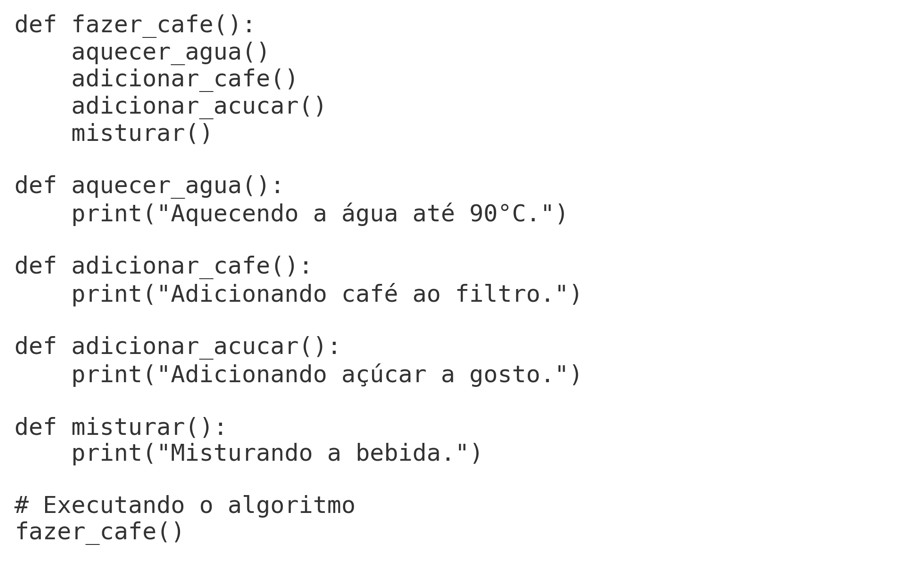
\includegraphics[width=0.75\linewidth]{Fig2.png}
%     \caption{Algoritmo de preparo de café representado em linguagem de programação.}
%     \label{fig2}
%     \source{Elaborado pelo autor via simulação por IA.}
% \end{figure}

Com base nessa \Cref{fig2}, vou explorar como os princípios da coesão textual se manifestam neste código, demonstrando de que maneira os elementos estruturais garantem a conexão entre as instruções e a progressão lógica do algoritmo.

\begin{enumerate}
    \item \emph{Referência e progressão}: Assim como um texto mantém sua continuidade por meio de referências anafóricas, o algoritmo se mantém coeso ao chamar funções previamente definidas. A função  \lstinline[language=Python]{fazer_cafe()} encapsula as etapas do processo e as referencia de maneira lógica.
    \item \emph{Substituição e evitação de redundância}: Em vez de repetir as instruções a cada vez que um café é preparado, o algoritmo substitui sequências inteiras de comandos por funções reutilizáveis (\lstinline[language=Python]{aquecer_agua()}, \lstinline[language=Python]{adicionar_cafe()}, etc.), garantindo economia textual e clareza.
    \item \emph{Encadeamento lógico (conjunção algorítmica)}: Assim como as conjunções coordenam ideias em um texto, a organização sequencial das chamadas de função define o fluxo do algoritmo, assegurando que as ações ocorram na ordem correta.
    \item \emph{Coesão lexical e nominalizações}: Assim como a escolha lexical influencia a legibilidade e coesão de um texto, a nomeação das funções (\lstinline[language=Python]{fazer_cafe}, \lstinline[language=Python]{aquecer_agua, misturar}) confere clareza semântica e contribui para a inteligibilidade do algoritmo, permitindo sua reutilização em diferentes contextos. Essa reutilização reforça a economia textual e a inteligibilidade do código, funcionando como uma estratégia de compressão informacional típica de textos bem coesos.
\end{enumerate}

Nesse código, observa-se que a função principal \lstinline[language=Python]{fazer_cafe()} organiza uma sequência de ações encapsuladas em outras funções menores. Essa organização revela uma forma de coesão discursiva e cognitiva na medida em que o encadeamento das etapas constrói uma progressão lógica e inteligível, tanto para a máquina que executa o código quanto para o ser humano que o lê ou o interpreta.

A coesão se manifesta, por exemplo, na substituição de trechos complexos por funções nomeadas \lstinline[language=Python]{aquecer_agua() e misturar()}, o que permite reutilização, clareza e legibilidade, efeitos equivalentes à substituição e à elipse em textos naturais. Além disso, há uma lógica de conjunção algorítmica, na qual a ordem das instruções constrói relações de causa, consequência e temporalidade. Do mesmo modo que uma conjunção como “então” marca consequência em um texto natural, a sequência de chamadas de função no código estabelece relações semânticas análogas. Essas estruturas não apenas formalizam a operação, mas produzem um efeito de continuidade textual, que orienta a ação e a compreensão.

Sob a ótica de \textcite{marcuschi2008}, a coesão também se dá em níveis multimodais. Em um ambiente digital real, esse algoritmo não se manifestaria apenas como texto codificado: seria visualizado em interfaces gráficas, acompanhado de botões, ícones ou comandos verbais, formando um fluxo interativo que articula diferentes linguagens. A coesão textual, nesse caso, emerge da integração entre os modos, código, imagem, gesto, e da relação interativa com o usuário, o que torna o algoritmo um texto sensível ao contexto e à recepção.

A textualidade algorítmica, portanto, não é um conjunto de propriedades estáticas do código, mas uma prática performativa que envolve design, leitura e interação. Como destaca \textcite{beaugrande1997}, os textos não são produtos fechados, mas atividades cognitivas e comunicativas inseridas em ecologias sociais e tecnológicas. O algoritmo, ao organizar ações com sentido e projetar respostas esperadas, participa de um processo de textualização que articula inferência, previsibilidade e adaptação, sendo coeso não por cumprir regras formais, mas por operar como um enunciado eficaz em redes sociotécnicas de significação, orientado por inferência, previsibilidade e interação.

Além disso, a repetição controlada (por laços de execução), os nomes simbólicos das funções e a substituição de comandos inteiros por abstrações reutilizáveis funcionam como estratégias de \emph{coesão cognitiva}, que favorecem a legibilidade e a previsibilidade do processo. Por exemplo, no trecho do código analisado, a função denominada \lstinline[language=Python]{verificarIdentidadeUsuario()} atua como um \emph{nome simbólico}, pois, em vez de descrever linha a linha o que o algoritmo faz para checar credenciais, o nome da função condensa cognitivamente esse conjunto de ações, ativando no leitor uma expectativa sobre sua finalidade.

Do mesmo modo, a criação de um módulo chamado autenticarViaBiometria(), em vez da repetição direta de seus comandos internos, exemplifica a \emph{substituição por abstração reutilizável}, tornando o código mais coeso e previsível ao permitir que a lógica da autenticação biométrica seja acionada por um único nome, mesmo que internamente envolva múltiplas etapas. Assim, a coesão algorítmica é menos uma exigência estrutural formal e mais um efeito de textualização, no qual operam escolhas de design, estratégias de programação e expectativas de interação. Essa leitura se afasta da ideia de texto como produto, e se alinha à concepção contemporânea de textualidade como processo cognitivo, social e situado \cite{koch2006,marcuschi2008}.

\section{Sentidos em linhas de código: coerência como inferência interativa}\label{sec-modelo}
Na concepção clássica da Linguística Textual, a coerência textual é entendida como a propriedade semântica que garante a inteligibilidade global do texto, organizando suas partes em torno de um sentido unitário. No entanto, como argumenta \textcite{koch2006}, a coerência não é uma característica interna ao texto, mas um efeito cognitivo construído por seus leitores ou usuários, com base em inferências, esquemas mentais e conhecimentos de mundo. Essa mudança de perspectiva é decisiva para analisar algoritmos como textos: o que os torna coerentes não é apenas a progressão lógica das instruções, mas sua capacidade de sustentar expectativas e fazer sentido em situações de uso que envolvem inferência, contexto e interação multimodal, como acontece nos algoritmos.

O algoritmo \lstinline[language=Python]{fazer_cafe()} exemplifica essa dimensão processual. Ele é coerente não porque cumpre um modelo formal de organização textual, mas porque, ao ser lido, seja pela máquina, seja por um humano que interpreta o código, permite antecipar etapas, acionar representações mentais e construir sentidos pragmáticos. Quando o leitor vê a função \lstinline[language=Python]{fazer_cafe()}, sabe que encontrará, na sequência, ações relacionadas ao preparo da bebida. A coerência decorre da ativação de conhecimentos prévios e da expectativa de um encadeamento lógico. Se uma instrução como \lstinline[language=Python]{ligar_televisao()} fosse inserida nesse ponto, a quebra de coerência seria evidente, não por erro técnico, mas por ruptura com a coerência pragmática construída na interação com o leitor do código.

Além disso, a coerência algorítmica também é multimodal e isso se aplica tanto ao modo como os algoritmos operam nas interfaces quanto à própria forma gráfica da linguagem de programação. Elementos como o uso do sublinhado (\_) para unir palavras como em \lstinline[language=Python]{adicionar_acucar()}, a estrutura dos parênteses (), a indentação para marcar blocos subordinados, a supressão de espaços, o uso de aspas para expressões textuais, e a disposição sequencial vertical não são neutros, mas são convenções visuais e formais que orientam a leitura e participam da construção de sentidos. Essas marcas funcionam como unidades significantes no interior do código e podem ser lidas como recursos de coerência visual e funcional, análogos a marcadores discursivos em textos naturais.

Em contextos digitais reais, a coerência se expande também para a dimensão interacional, pois os algoritmos só fazem sentido quando suas respostas se alinham às expectativas dos usuários em tempo real. Um sistema que prepara café por comando de voz, por exemplo, deve interpretar o \textit{input}, executar ações encadeadas e retornar feedback compreensível (auditivo, visual ou textual). Esse processo envolve coerência pragmática: o algoritmo precisa “conversar” com o ambiente de uso. Nesse caso, a coerência não é garantida por estrutura interna, mas pela responsividade do algoritmo às práticas comunicativas dos sujeitos.

\textcite{beaugrande1997} já apontava que a coerência textual emerge de redes de interação comunicativa e de acesso ao conhecimento, e não de propriedades internas ao texto. No caso dos algoritmos, isso significa que sua coerência resulta de múltiplos fatores, tais como: o funcionamento lógico do código, as inferências ativadas pelo usuário, a estrutura visual da linguagem e a adequação situacional. Desse modo, é possível afirmar que o algoritmo é coerente não por cumprir uma forma canônica, mas porque ativa, negocia e sustenta sentidos em ecossistemas de linguagem mediados por máquinas, interfaces e humanos.

Além disso, a coerência algorítmica também implica que as instruções dialoguem entre si e cumpram um propósito dentro de um contexto específico. O exemplo da receita de café, estruturada como algoritmo, ilustra como a coerência textual se manifesta no código, pois ela organiza as instruções de modo lógico e garante sua inteligibilidade.

\begin{enumerate}
    \item Unidade temática e continuidade do propósito: A coerência de um texto depende de sua unidade temática, ou seja, de um eixo semântico que organize suas partes em torno de um mesmo objetivo. No exemplo acima, todas as instruções convergem para a preparação do café. Se, subitamente, o código incluísse uma função como \lstinline[language=Python]{desligar_luz_cozinha()} ou ligasse a televisão, a coerência seria rompida, pois a sequência perderia sua progressão lógica.
    \item Progressão semântica e relação hierárquica das partes: A coerência textual pressupõe que as ideias se organizam de forma progressiva e interdependente. No código, a função principal \lstinline[language=Python]{fazer_cafe()} estrutura a sequência de ações e mantém a lógica hierárquica: ela chama outras funções (\lstinline[language=Python]{aquecer_agua()},\lstinline[language=Python]{adicionar_cafe()}, \lstinline[language=Python]{adicionar_acucar()}, \lstinline[language=Python]{misturar()}), estabelecendo um fluxo compreensível. Se a ordem das funções fosse alterada de maneira ilógica, como misturar o café antes de adicionar a água, a coerência do processo seria comprometida.
    \item Causalidade e relações lógicas: Como qualquer texto deve apresentar relações causais e temporais que tornem sua interpretação possível, um algoritmo coerente precisa respeitar relações lógicas de causa e consequência. No código, a necessidade de aquecer a água antes de adicioná-la ao café segue um princípio lógico que, se violado, comprometeria o funcionamento da receita para um café quente. Esse aspecto é análogo à coerência textual, na qual sentenças desconectadas logicamente dificultam a compreensão do discurso.
    \item Predição e interpretabilidade: Para que um texto seja coerente, ele deve permitir que o leitor antecipe o desenvolvimento das informações com base no que já foi apresentado. Da mesma forma, um algoritmo coerente deve ser interpretável de maneira lógica. Ao ler \lstinline[language=Python]{fazer_cafe()}, um leitor que compreende a estrutura do código pode prever quais etapas virão a seguir, assim como um leitor experiente pode antecipar a conclusão de um parágrafo bem estruturado.
\end{enumerate}
    
Para serem executáveis e compreensíveis, os códigos devem apresentar unidade temática, progressão lógica, relações causais definidas e interpretabilidade, características essenciais a qualquer texto coerente. Um algoritmo sem lógica, assim como um texto incoerente, torna-se ineficaz. Essa constatação reforça a tese central deste ensaio segundo a qual algoritmos são textos estruturados que organizam significados e ações com base em uma lógica inteligível e situada.

\section{Interfaces que persuadem: a textualidade algorítmica em ação}\label{sec-organizacao}
Ao observar algoritmos como os de recomendação de conteúdo em plataformas de \textit{streaming}, não é mais suficiente aplicar uma lista de critérios como se fossem parâmetros estáticos de análise textual. A textualidade não é um conjunto de propriedades formais do texto, mas um processo emergente de construção de sentido, situado em contextos de produção, circulação e recepção \cite{koch2006,marcuschi2008,beaugrande1997}. É a partir dessa concepção que analiso o algoritmo de recomendação, não como uma estrutura codificada que possui textualidade, mas como um texto que acontece na interação com o usuário e na ativação de inferências, expectativas e experiências multimodais, em tempo real.

O que um algoritmo recomenda não é apenas conteúdo, mas uma ordem de visibilidade, uma escrita silenciosa que projeta sentidos, define acessos e organiza experiências. Desse modo, o algoritmo de recomendação não apenas lê dados, mas escreve o mundo a partir deles, projetando significados que moldam a experiência digital. Para aprofundar essa discussão, elaboro a seguir uma simulação de algoritmo de recomendação de conteúdo em plataformas de \textit{streaming}, sistemas que, mais do que executar comandos, atuam discursivamente ao organizar experiências, persuadir escolhas e construir sentidos em ambientes digitais.

Este exemplo, embora fictício (\Cref{fig3}), ilustra como a textualidade algorítmica se materializa em práticas situadas, multimodais e interacionais.


\begin{lstlisting}[language=Python, label=fig3, caption={Exemplo de Algoritmo: recomendação em plataformas de \textit{streaming}.}, source={Elaborado pelo autor via simulação por IA.}]
def recomendar_conteudo(usuario):
    preferencias = obter_preferencias(usuario)
    historico = obter_historico_visualizacoes(usuario)
    tendencias = obter_tendencias_globais()

    sugestoes = gerar_sugestoes(preferencias, historico, tendencias)

    print(f"Olá, {usuario}! Recomendamos para você: {sugestoes}")

def obter_preferencias(usuario):
    return ["ação", "ficção científica", "drama"]

def obter_historico_visualizacoes(usuario):
    return ["Matrix", "Blade Runner", "O Senhor dos Anéis"]

def obter_tendencias_globais():
    return ["Duna", "Interestelar", "The Batman"]

def gerar_sugestoes(preferencias, historico, tendencias):
    recomendacoes = []
    for filme in tendencias:
        if any(genero in filme for genero in preferencias): 
            recomendacoes.append(filme)
    return recomendacoes if recomendacoes else ["Confira nosso catálogo!"]

# Executando o algoritmo para um usuário fictício
recomendar_conteudo("João")
\end{lstlisting}
% \begin{figure}[h!]
%     \centering
%     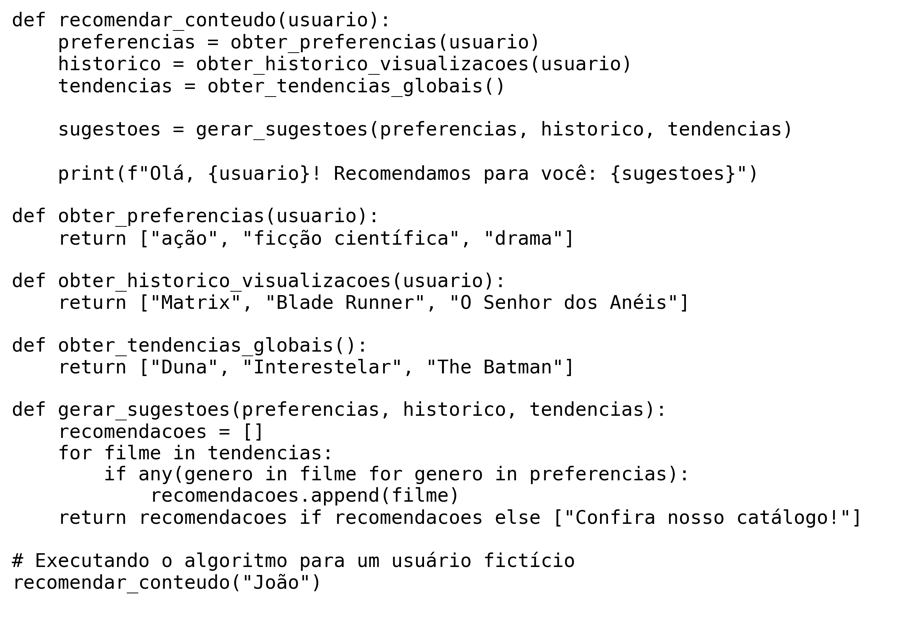
\includegraphics[width=0.75\linewidth]{Fig3.png}
%     \caption{Exemplo de Algoritmo: recomendação em plataformas de \textit{streaming}.}
%     \label{fig3}
%     \source{Elaborado pelo autor via simulação por IA.}
% \end{figure}

Não se trata de aplicar uma lista de critérios a um objeto técnico, mas de ler o algoritmo como uma textualidade emergente, que se constrói na interface com o usuário, na forma gráfica do código, nas inferências ativadas, nas respostas comunicacionais que produz. A textualidade, aqui, é uma prática e o algoritmo, um texto que age no mundo.

O algoritmo, no exemplo simulado, tem como função principal \lstinline[language=Python]{recomendar_conteudo(usuario)}. Essa função, embora pareça apenas uma instrução técnica, participa de uma pragmática algorítmica, pois ela é um gesto discursivo que propõe ao usuário uma continuidade narrativa com base em dados prévios. O sistema não apenas executa comandos, mas lê o usuário, interpretando suas preferências, e responde discursivamente, adaptando sua forma de agir. Isso é textualidade interacional.

A função \lstinline[language=Python]{gerar_sugestoes(preferencias, historico, tendencias)} articula diferentes camadas de inferência e me permite afirmar, segundo \textcite{koch2006}, que representa uma operação cognitiva na medida em que o sistema ativa esquemas mentais baseados em hábitos anteriores, cruza com padrões coletivos e entrega um enunciado personalizado. Essa personalização não é apenas decorativa, pois ela performa sentido discursivo. O sistema exibe sugestões e constrói uma narrativa personalizada, sustentada por inferências e esquemas mentais que articulam memória e predição.

Assim, quando o sistema escreve \lstinline[language=Python]|print(f"Olá, {usuario}! Recomendamos para você: {sugestoes}"|), ele adota uma voz discursiva que simula diálogo, aproximando-se das estratégias dos textos publicitários, como bem observa \textcite{marcuschi2008}, ao mostrar que o texto se configura como uma instância de negociação constante de sentidos.

Essa negociação também é multimodal, pois a recomendação não se apresenta apenas como texto codificado, já que ela é também visual, sonora, afetiva e até temporal. A disposição gráfica dos \textit{cards} na interface, o tipo de imagem que representa o conteúdo sugerido, a ordem em que as opções aparecem e os sons que acompanham a recomendação fazem parte da textualidade do algoritmo. O código \lstinline[language=Python]{print()} que aparece no exemplo é apenas um marcador de um processo maior de produção discursiva sensorial. Trata-se de uma textualidade sensorial e performativa, que atua no entrelaçamento de formas, tempos e afetos.

O uso de sintaxes como \lstinline[language=Python]{obter_historico_visualizacoes(usuario)} e \lstinline[language=Python]{obter_tendencias_globais()} revela a intertextualidade algorítmica: o algoritmo é um texto como qualquer outro, que também pode se construir a partir de outros textos, dados anteriores, padrões coletivos, discursos já circulados. Essa articulação entre o individual e o coletivo configura o que \textcite{beaugrande1997} chama de produção textual em redes de acesso ao conhecimento. Nesse sentido, a textualidade algorítmica atualiza o princípio de intertextualidade como rede de discursos que se reconfiguram em contextos específicos, como também propõe \textcite{beaugrande1997}.

Além disso, a própria linguagem de programação empregada é portadora de textualidade gráfica e visual. Elementos como (), \_, a ausência de espaços, o uso de palavras reservadas como def, print, return, todos esses aspectos têm valor semântico e funcionam como marcadores visuais e cognitivos. O leitor de código, seja humano ou máquina, compreende a estrutura textual por meio dessas convenções, que atuam como uma gramática multimodal da programação.

É importante salientar que a textualidade desse algoritmo não está dada, na medida em que ela é construída na relação com o leitor/usuário, que pode aceitar, rejeitar, ignorar ou interagir com a recomendação. A textualidade, nesse caso, não é uma propriedade do algoritmo, mas uma atividade social e comunicativa que envolve cognição, contexto e resposta. A estrutura do código é apenas a base sobre a qual se ergue o texto algoritmo, que é um enunciado performativo que opera na economia da atenção, na estética da interface e nos hábitos de consumo digital em tempos de inteligência artificial. O algoritmo, portanto, age como um texto que não apenas responde, mas convoca, moldando aquilo que é possível ver, desejar e escolher.

Dizer que algoritmos são textos não significa aplicar-lhes um \textit{checklist} de critérios fixos, mas reconhecer que eles participam de práticas discursivas que constroem sentidos, organizam a interação e moldam a experiência social dos usuários. Na Linguística Textual, é defendido que o texto é uma ocorrência situada, processual e multimodal, não um produto acabado, mas uma atividade cognitiva e interacional. Com base nessa abordagem, analiso a seguir o mesmo algoritmo de recomendação em plataformas de \textit{streaming} como um texto performativo, cujas dimensões de intencionalidade, aceitabilidade, informatividade, situacionalidade e intertextualidade se articulam não como propriedades internas, mas como efeitos emergentes da textualização algorítmica.

\section{Textualidade emergente: dimensões discursivas do algoritmo}\label{sec-organizacao-latex}
\subsection{Intencionalidade como ação discursiva}
A textualidade não se inicia no conteúdo, mas na finalidade. O algoritmo \lstinline[language=Python]{recomendar_conteudo(usuario)} atua com uma intencionalidade explícita: engajar o usuário por meio de recomendações personalizadas. Essa função performa um gesto comunicativo que, embora programado, busca simular diálogo, construir empatia e sugerir continuidade narrativa, traços típicos dos textos publicitários. Nesse caso, o algoritmo assume um papel enunciativo persuasivo, que simula interlocução para capturar atenção e orientar escolhas. Como destaca \textcite{marcuschi2008}, textos em ambientes digitais mobilizam estratégias de interpelação que os tornam discursivamente orientados, e esse é justamente o caso aqui, uma vez que não se trata de processar dados frios, mas de propor escolhas, influenciar gostos e manter o sujeito conectado à plataforma.

\subsection{Aceitabilidade como negociação interativa}\label{sec-titulo}
A textualidade algorítmica só se realiza se o leitor, neste caso, o usuário, aceitar a mensagem como válida, útil e pertinente. Isso envolve diferentes camadas, tais como a personalização da experiência (\lstinline[language=Python]{gerar_sugestoes(...)}), a clareza na apresentação das recomendações (\lstinline[language=Python]{print(...)}) e a conformidade com os hábitos do usuário (\lstinline[language=Python]{obter_historico_visualizacoes(...)}). A aceitabilidade, assim, não é um atributo do código, mas um efeito discursivo negociado entre o sistema e o sujeito, que decide, a cada clique ou rejeição, se a leitura proposta pelo algoritmo faz sentido. Como em qualquer texto, há ruído, recusa, adaptação. E o próprio algoritmo incorpora essa dimensão, pois ele aprende com o comportamento do usuário e modifica suas sugestões, uma textualidade que se reconfigura continuamente a partir do gesto interpretativo do outro, como observa \textcite{koch2006} sobre os processos inferenciais da leitura.

\subsection{Informatividade como equilíbrio entre familiaridade e novidade}\label{sec-autores}
A função \lstinline[language=Python]{gerar_sugestoes(...)} opera sobre um campo tensionado entre o já conhecido e o ainda não visto. A textualidade aqui se constrói na capacidade do sistema de introduzir o novo sem romper com o repertório do usuário. Filmes que ainda não foram assistidos, mas que compartilham gêneros, diretores ou atmosferas com o histórico do usuário, são estrategicamente posicionados como “descobertas guiadas”. A informatividade algorítmica, assim, é relacional e situada na medida em que depende do contexto de uso, do acúmulo de interações e da capacidade do sistema de oferecer surpresa com segurança, como um bom texto, que informa sem dispersar. Essa é uma operação cognitiva refinada, que exige inferência, previsão e atualização permanente dos dados. Como em todo texto que informa com eficácia, o algoritmo precisa medir o grau de informatividade para não dispersar nem entediar, ativando, assim, um equilíbrio discursivo próprio.

\subsection{Situacionalidade como textualidade contextualizada}\label{sec-idioma}
A textualidade de um algoritmo de recomendação não se realiza no vazio, já que ela depende do ambiente técnico, do dispositivo de acesso, do momento de uso e do contexto cultural. Recomendar comédias românticas em pleno Halloween pode gerar ruído. Sugerir filmes longos num celular pode comprometer a experiência. A função \lstinline[language=Python]{obter_tendencias_globais()} e a consideração por eventos sazonais mostram que o algoritmo reage ao mundo, e isso o torna um texto sensível ao tempo, ao lugar e à situação. Como destaca \textcite{marcuschi2008}, a situacionalidade não é pano de fundo, mas constitutiva da produção de sentido. O algoritmo, nesse caso, atua como um texto oportuno, que se ajusta às circunstâncias comunicativas para permanecer relevante e, ao fazê-lo, performa um texto tempestivo, que lê o mundo antes de escrever suas respostas.

\subsection{Intertextualidade como rede semântica em movimento}\label{sec-resumo}
Nenhum texto nasce do zero, e isso também vale para os algoritmos. A função \lstinline[language=Python]{obter_historico_visualizacoes(...)} revela como o sistema se ancora em experiências anteriores para produzir novas recomendações. Nesse sentido, é possível afirmar que os algoritmos são intertextuais por natureza, pois reprocessam dados, ecoam padrões, dialogam com tendências, simulam formas narrativas conhecidas.

A própria linha \lstinline[language=Python]|print(f"Olá, {usuario}! Recomendamos para você: {sugestoes}"|) reproduz o tom conversacional típico de discursos publicitários, estabelecendo pontes discursivas com práticas de enunciação já socialmente consolidadas. Assim, o algoritmo inscreve-se numa cadeia discursiva contínua, em que cada recomendação ecoa repertórios prévios e atua como atualização performativa do já-dito. Isso reforça o argumento de que a textualidade algorítmica é processual, contínua e hipertextual, pois ela atua em rede, moldando sentidos em função de repertórios e sistemas que a precedem e a ultrapassam.

As dimensões aqui analisadas mostram que o algoritmo de recomendação é muito mais do que um sistema técnico, uma vez que ele atua como um texto porque organiza sentidos, articula formas de interação e atua discursivamente no mundo das digitalidades. Sua textualidade não é algo que se verifica a partir de critérios fechados, mas algo que se realiza na prática, na leitura, na resposta, no afeto, no clique. Alinhado à concepção contemporânea da Linguística Textual, este ensaio não propõe que o algoritmo possui textualidade, mas que ele a exerce, performando significados em ambientes interacionais, cognitivos e multimodais.

Todas essas análises convergem para uma concepção de textualidade que é, ao mesmo tempo, discursiva, interacional, multimodal e situada. Ao aplicar os fatores de textualidade aos algoritmos, este ensaio não os trata como um \textit{checklist} normativo, mas como operadores discursivos que emergem em situações comunicativas específicas, conforme apontam \textcite{koch2006,marcuschi2008}. A proposta de que “o algoritmo é um texto” sustenta-se, assim, não apenas na correspondência estrutural com os textos naturais, mas em sua atuação cognitiva e social como um enunciado performativo, que regula sentidos, interações e exclusões e, por isso mesmo, deve ser lido criticamente como texto que age no e sobre o mundo.

\section{Conclusão}\label{sec-secoes}
Ao longo deste ensaio, afirmei que os algoritmos podem e devem ser lidos como textos performativos. A partir de uma concepção contemporânea de textualidade, que os entende como práticas situadas, interacionais, multimodais e cognitivas \cite{koch2006,marcuschi2008,beaugrande1997}, demonstrei que a linguagem algorítmica não é neutra nem puramente técnica, já que ela organiza sentidos, regula interações e molda experiências sociais.

A leitura textual dos algoritmos, proposta aqui, desloca o foco das estruturas formais para os efeitos emergentes de significação. A análise de algoritmos simulados, como o preparo de café ou o sistema de recomendação em plataformas de \textit{streaming}, mostrou que fatores como coesão, coerência, intencionalidade, aceitabilidade, informatividade, situacionalidade e intertextualidade se manifestam na forma de processos dinâmicos de textualização, mediados por código, interface, contexto e uso. Os algoritmos não apenas executam instruções, pois também produzem discursos.

Essa abordagem não é apenas analítica, mas política. Se os algoritmos são textos, então operam como gramáticas do mundo digital, projetando narrativas que distribuem visibilidade, acesso e oportunidades. Como adverte \textcite{crawford2021atlas}, a inteligência artificial é um artefato político, sustentado por infraestruturas de poder, que seleciona quais dados importam, como são processados e com quais efeitos. Nesse sentido, os algoritmos escrevem sobre nós e, muitas vezes, contra nós.

\textcite{pasquale2015black} mostra que essas “caixas-pretas” algorítmicas eclipsam as lógicas de decisão que afetam crédito, saúde, segurança e trabalho, operando como sistemas de exclusão automatizada contra comunidades racializadas. \textcite{noble2021}, por sua vez, expõe como algoritmos reforçam estereótipos raciais e de gênero, atuando como arquiteturas da discriminação e misoginia. Desse modo, esses sistemas, longe de serem neutros, reconfiguram desigualdades históricas em tempo real.

No caso do racismo algorítmico, os algoritmos são genuínos textos, codificando e institucionalizando hierarquias \cite{araujo2024_microagressoes,araujo2024_racismo_ia}. Quando treinados com dados enviesados, algoritmos de reconhecimento facial, por exemplo, erram mais com rostos negros \cite{buolamwini2018}, algoritmos de crédito penalizam populações vulnerabilizadas \cite{loya2022} e sistemas de recrutamento automatizado excluem perfis que fogem do padrão hegemônico. Essas operações discursivas e computacionais expressam o que denominei necroalgoritmização \cite{araujo2025_necroalgoritmizacao}, isto é, a organização algorítmica da exclusão, do silenciamento e da morte social.

Reconhecer que algoritmos são textos nos convida a uma ética da leitura crítica. Assim como textos podem ser contestados, reescritos e democratizados, os algoritmos devem ser interpretados como dispositivos de poder simbólico e material. Isso implica disputar suas linguagens, desvelar suas ideologias e reivindicar metodologias de auditabilidade, reescrita e justiça digital.

A proposta aqui defendida amplia os horizontes da Linguística Textual ao incorporar os algoritmos como objetos textuais e políticos. Se todo texto performa sentidos e disputas, os algoritmos, enquanto textos computacionais, integram regimes discursivos que estruturam o mundo contemporâneo. Desse modo, a interseção entre linguagem e tecnologia abre caminho para novos paradigmas de leitura, nos quais a crítica textual encontra a governança algorítmica.

Mais do que uma metáfora, afirmar que o algoritmo é um texto é reivindicar o direito de lê-lo, interpretá-lo e reescrevê-lo. É afirmar que a inteligência artificial não pode ser apenas eficiente, mas deve ser inteligível e socialmente responsável. Os estudos futuros que partirem dessa hipótese poderão desenvolver metodologias críticas de análise, escuta e resistência, valorizando formas contra-hegemônicas de programar e imaginar futuros possíveis.


\printbibliography\label{sec-bib}
% if the text is not in Portuguese, it might be necessary to use the code below instead to print the correct ABNT abbreviations [s.n.], [s.l.]
%\begin{portuguese}
%\printbibliography[title={Bibliography}]
%\end{portuguese}


\end{document}

